\chapter{Results}\label{chapter:results} \

In Chapter~\ref{chapter:results} we will introduce
the results of the experiments presented in Chapter
~\ref{chapter:implementation}. The results will be presented
per dataset. Each dataset contains two graphs related to
the model accuracy on the clean test set for noisy and
noiseless models. Additionally, two more graphs are
introduced to portray the effect of the adversarial
attacks on the noiseless \ac{qml} model, one for each
attack with increasing attack strengths. Finally, two
graphs for each of the six noise models are provided.
These last graphs will provide insights of the effects
of the diverse quantum noise sources with different noise 
magnitudes on the adversarial accuracy of both adversarial
attacks. \

In Section~\ref{section:iris-eval} the results from
the Iris dataset are shown. In Section~\ref{section:diabetes-eval}
the results from the \ac{pid} dataset follow. Moreover,
in Section~\ref{section:breast-cancer-eval} the outcomes
for the Wisconsin Breast Cancer dataset can be found.
Lastly, the experiments' outcomes from the Plus-Minus dataset
are provided in Section~\ref{section:plus-minus-eval}. \

\section{Iris Dataset}\label{section:iris-eval} \

The results obtained from training the noisy and noiseless
\ac{qml} models on the Iris dataset can be found in Subsection
~\ref{subsection:iris-noisy-acc}. Moreover, the outcomes
of both adversarial attacks will be presented in Subsection
~\ref{subsection:iris-adv-acc}. Finally, the evaluation
of the noisy models against the adversarial attacks can
are presented in Subsection~\ref{subsection:iris-noisy-adv-acc}. \

\subsection{Noisy Models Accuracy}\label{subsection:iris-noisy-acc} \

In Figure~\ref{fig:iris-12} we can observe the results
from the training of noiseless and noisy \ac{qml} models
for the Iris test dataset. The noiseless baseline model accuracy
can be found on both graphs at the y-intercept, which in
this case is of \(100\%\). We note in Subfigure~\ref{fig:iris1}
that for the Iris dataset there are no perceptible
repercussions on the model accuracy when training with
coherent noise and remains the same as the noiseless
baseline performance. \

Nevertheless, for incoherent noise models in Subfigure
~\ref{fig:iris2} we can already observe a decrease in
model accuracy for certain noise models. For depolarizing
noise and bit-flip induced noise we notice the same behavior
as with coherent noise, remaining constant throughout
the different noise magnitudes and obtaining the same
performance as the noiseless model. \

Regarding phase damping noise, the model performance
marginally decreases the accuracy to \(97\%\) starting at
\(8\%\) noise probability. For phase-flip induced noise
the model performance slightly decreases in comparison
to phase damping noise to \(90\%\) at \(6\%\) noise probability
until the accuracy decreases to \(86\%\) at \(10\%\). Moreover,
for amplitude damping noise we can appreciate that the model
performance oscilates significantly starting \(4\%\) noise
probability. Furthermore, amplitude damping \ac{qml}
model's accuracy is significantly lower than other noiseless
and noisy models, reaching \(50\%\) accuracy at \(10\%\)
noise probability. \

\begin{figure}[!h]
  \centering

  \begin{subfigure}{0.45\textwidth}
      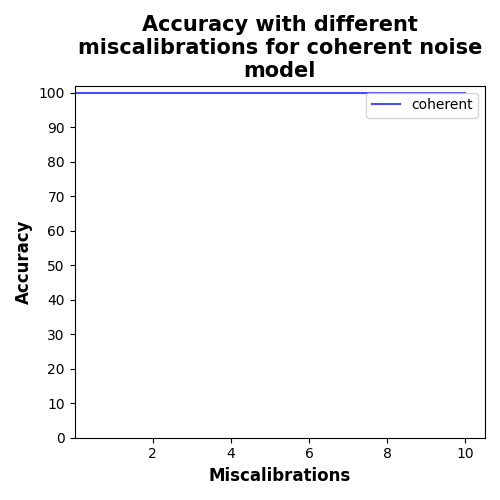
\includegraphics[width=\linewidth]{figures/evaluation_results/iris/pqc/figures/accuracy-coherent.png}
      \subcaption{Coherent noise model's accuracy.}
      \label{fig:iris1}
  \end{subfigure} \qquad
  \begin{subfigure}{0.45\textwidth}
      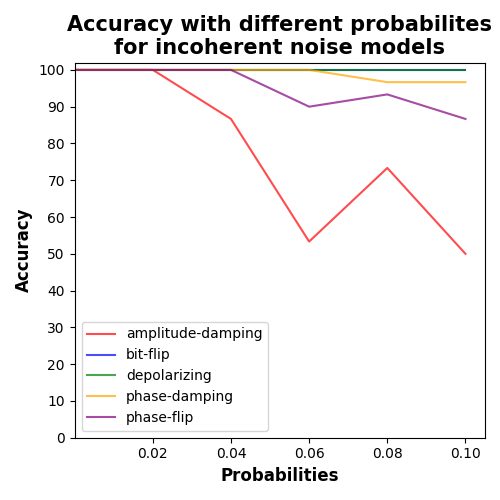
\includegraphics[width=\linewidth]{figures/evaluation_results/iris/pqc/figures/accuracy-incoherent.png}
      \subcaption{Incoherent noise models' accuracy.}
      \label{fig:iris2}
  \end{subfigure}

  \caption{\ac{vqa}'s accuracy on the Iris clean test dataset.}
  \label{fig:iris-12}
\end{figure} \

\subsection{Adversarial Accuracy}\label{subsection:iris-adv-acc} \

In Figure~\ref{fig:iris-34} we introduce the effects of the
adversarial attacks on the accuracy of the noiseless \ac{qml}
model. As expected, we can observe that for both adversarial
techniques the performance of the model decreases with increasing
attack strength. For the \ac{fgsm} technique in Subfigure~\ref{fig:iris3}
we notice a stark accuracy decrease until it stabilizes to around
\(50\%\) after \(0.5\) attack strength. Furthermore, in Subfigure
~\ref{fig:iris4} for the \ac{pgd} technique we see a lesser performance
decrease that stabilizes to around \(70\%\) after \(0.5\) attack strength. 
That \ac{fgsm} has a bigger performance impact than \ac{pgd} is expected
as \ac{fgsm}'s perturbations tend to be bigger in magnitude and more
disruptive to the input. \

\begin{figure}[!h]
  \centering

  \begin{subfigure}{0.45\textwidth}
      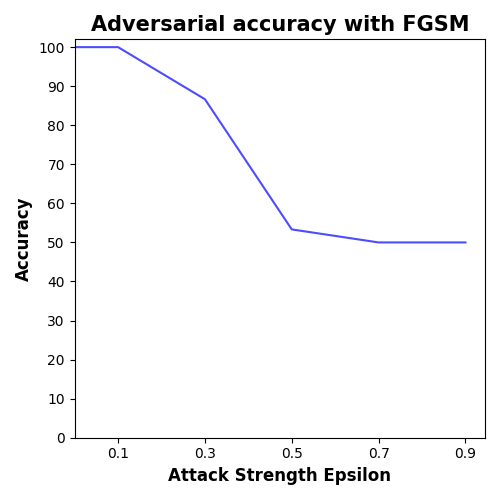
\includegraphics[width=\linewidth]{figures/evaluation_results/iris/pqc/figures/none-fgsm.png}
      \subcaption{Noiseless model's \ac{fgsm} adversarial accuracy.}
      \label{fig:iris3}
  \end{subfigure} \qquad
  \begin{subfigure}{0.45\textwidth}
      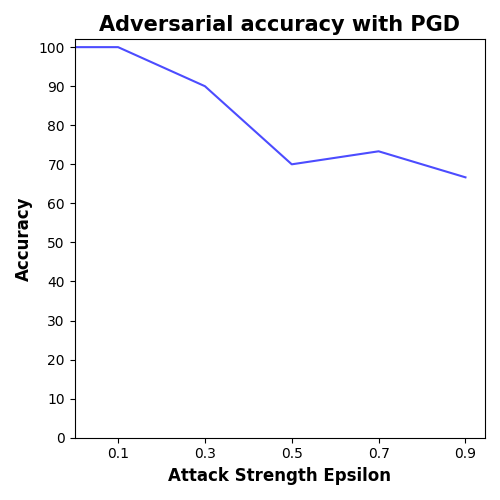
\includegraphics[width=\linewidth]{figures/evaluation_results/iris/pqc/figures/none-pgd.png}
      \subcaption{Noiseless model's \ac{pgd} adversarial accuracy.}
      \label{fig:iris4}
  \end{subfigure}

  \caption{\ac{vqa}'s accuracy on the adversarial Iris test dataset.}
  \label{fig:iris-34}
\end{figure} \

\subsection{Noisy Models Adversarial Accuracy}\label{subsection:iris-noisy-adv-acc} \

In this subsection we introduce the results from performing
the adversarial attacks on the noisy models with different noise
magnitudes for the Iris dataset. In each graph the color gray
represents the baseline adversarial accuracy obtained by the
noiseless model. \

In Figure~\ref{fig:iris-56} we present the outcomes from the amplitude
damping noisy models evaluation. For \ac{fgsm} in Subfigure~\ref{fig:iris5}
we note that the model with \(2\%\) noise probability obtains the same
performance as the noiseless model. Furthermore, we observe that an
increase in noise probability when training in general does not equate
to a worse adversarial accuracy at lower attack strengths, as the model
with \(8\%\) noise probability performs better than the one with \(6\%\)
noise probability. Nevertheless, once the attack strength reaches a
value of \(0.9\) all the models perform equally, converging to \(50\%\)
accuracy. \

\begin{figure}[!h]
  \centering

  \begin{subfigure}{0.45\textwidth}
      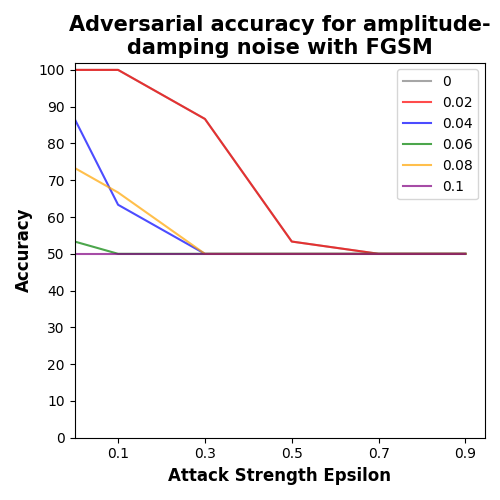
\includegraphics[width=\linewidth]{figures/evaluation_results/iris/pqc/figures/amplitude-damping-fgsm.png}
      \subcaption{Amplitude damping noise model's \ac{fgsm} adversarial accuracy.}
      \label{fig:iris5}
  \end{subfigure} \qquad
  \begin{subfigure}{0.45\textwidth}
      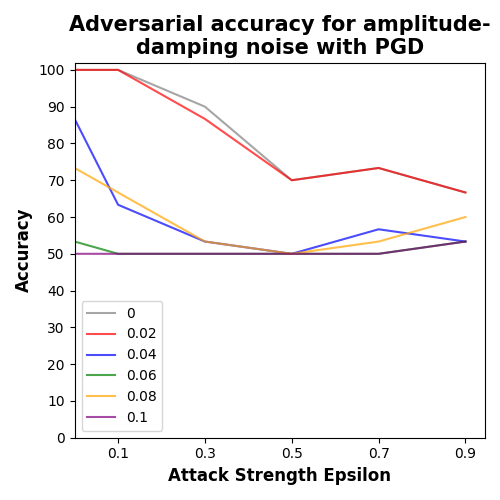
\includegraphics[width=\linewidth]{figures/evaluation_results/iris/pqc/figures/amplitude-damping-pgd.png}
      \subcaption{Amplitude damping noise model's \ac{pgd} adversarial accuracy.}
      \label{fig:iris6}
  \end{subfigure}
  \caption{Amplitude damping noise models' accuracy on the adversarial Iris test dataset.}
  \label{fig:iris-56}
\end{figure} \

In Subfigure~\ref{fig:iris6} we introduce the results from the \ac{pgd}
attack on the amplitude damping noisy models. As with the \ac{fgsm} attack
we can observe that the best performing model (close to the noiseless
model's performance) is the one with the smallest noise probability. Also,
we can note that increasing noise probability does not equal a direct
decrease in adversarial accuracy at lower attack strengths. Nevertheless,
noisy models in general perform significantly worse than the noiseless
model. Interestingly, when the attack strength surpasses \(0.5\), all
the noisy models (with the exception of the model with \(2\%\) noise
probability) perform slightly better than at lower attack strengths. \

In Figure~\ref{fig:iris-78} we present the outcomes from the bit-flip
noisy models evaluation. For \ac{fgsm} in Subfigure~\ref{fig:iris7}
we note that there are some models (\(2\%, 4\%, 10\%\)) performing
better than the noiseless model, while others (\(6\%, 8\%\)) have
a lower or equal adversarial accuracy throughout the different
attack strengths. While the model trained with \(10\%\) noise
probability performs the best against attack strength's lower
than \(0.7\), the adversarial accuracy drops to around \(33\%\)
(the lowest recorded accuracy) at an attack strength of \(0.9\). \

\begin{figure}[!h]
  \centering

  \begin{subfigure}{0.45\textwidth}
      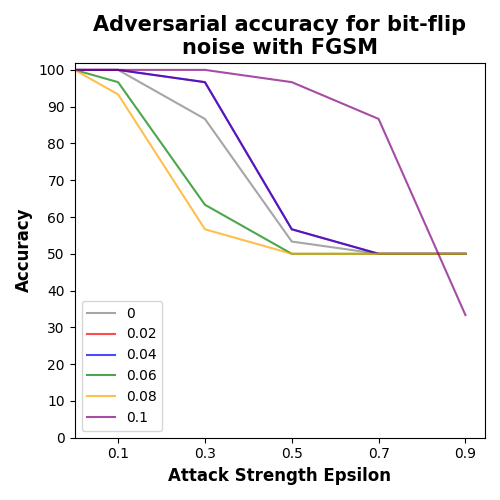
\includegraphics[width=\linewidth]{figures/evaluation_results/iris/pqc/figures/bit-flip-fgsm.png}
      \subcaption{Bit-Flip noise model's \ac{fgsm} adversarial accuracy.}
      \label{fig:iris7}
  \end{subfigure} \qquad
  \begin{subfigure}{0.45\textwidth}
      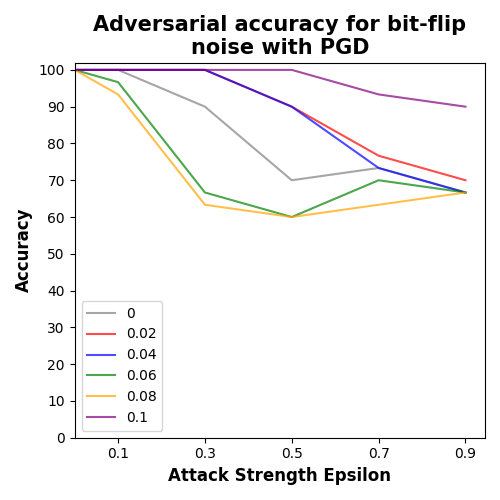
\includegraphics[width=\linewidth]{figures/evaluation_results/iris/pqc/figures/bit-flip-pgd.png}
      \subcaption{Bit-Flip noise model's \ac{pgd} adversarial accuracy.}
      \label{fig:iris8}
  \end{subfigure}
  \caption{Bit-Flip noise models' accuracy on the adversarial Iris test dataset.}
  \label{fig:iris-78}
\end{figure} \

In Subfigure~\ref{fig:iris8} we introduce the results from the \ac{pgd}
attack on the bit-flip noisy models. Similar to the \ac{fgsm} performance,
the models with noise probability (2\%, 4\%, and 10\%) perform better or equal
than the baseline noiseless adversarial accuracy. Nevertheless, the stark
performance drop from the model trained with 10\% noise probability
at 0.9 attack strength does not occur in this case. Furthermore, analogous
to the \ac{fgsm} results, the models trained with (6\% and 8\%) noise
probability perform worse than the noiseless model. However, with attack
strengths higher than 0.5, these models actually see a slight performance
increase to match the baseline model at 0.9 attack strength. \

In Figure~\ref{fig:iris-910} we present the outcomes from the coherent
noisy models evaluation. For \ac{fgsm} in Subfigure~\ref{fig:iris9}
we note that all the noisy models perform better than the noiseless
models throught almost all of the attack strength range. Only at 
attack strength 0.9 do the models with a misconfiguration of 2 and
4 degrees have a marginally lower accuracy than the noiseless model's
accuracy. In this specific case, there seems to be a slight correlation
between model robustness and degree misconfiguration, where the
higher the misconfiguration degree leads to a more robust model. The
two models with the highest coherent noise (8 and 10 degrees) achieve
an adversarial accuracy of around 96\% at the highest attack strength. \

\begin{figure}[!h]
  \centering

  \begin{subfigure}{0.45\textwidth}
      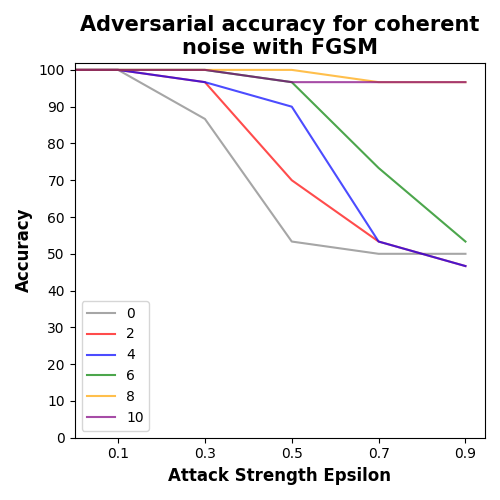
\includegraphics[width=\linewidth]{figures/evaluation_results/iris/pqc/figures/coherent-fgsm.png}
      \subcaption{Coherent noise model's \ac{fgsm} adversarial accuracy.}
      \label{fig:iris9}
  \end{subfigure} \qquad
  \begin{subfigure}{0.45\textwidth}
      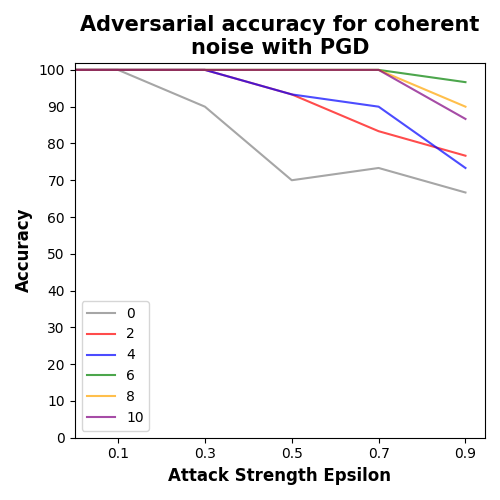
\includegraphics[width=\linewidth]{figures/evaluation_results/iris/pqc/figures/coherent-pgd.png}
      \subcaption{Coherent noise model's \ac{pgd} adversarial accuracy.}
      \label{fig:iris10}
  \end{subfigure}
  \caption{Coherent noise models' accuracy on the adversarial Iris test dataset.}
  \label{fig:iris-910}
\end{figure} \

In Subfigure~\ref{fig:iris10} we introduce the results from the \ac{pgd}
attack on the coherent noisy models. Comparable to the results from the
\ac{fgsm} evaluation, all the coherent noisy models perfom better than
the baseline noiseless model benchmark. Furthermore, the coherent noisy
models with a lower misconfiguration degree obtain a lower adversarial
accuracy than the models with a higher noise disturbance. Thus, we can
derive a slight correlation with the degree of misconfiguration and the
adversarial accuracy. \

In Figure~\ref{fig:iris-1112} we present the outcomes from the depolarizing
noisy models evaluation. For \ac{fgsm} in Subfigure~\ref{fig:iris11}
we note that all the noisy models but the one with 2\% noise probability
perform at equal or better than the noiseless benchmark until the attack
strength 0.7 is reached. The model with 4\% noise probability is the best
model in this range. However, this model's adversarial accuracy significantly
drops to the lowest value recorded at around 26\% with attack strength's
higher than 0.7. While most of the noisy models have a higher adversarial
accuracy than the noiseless model throughout the attack strength range,
no direct correlation can be drawn between the noise probability and the
model's robustness. \

\begin{figure}[!h]
  \centering

  \begin{subfigure}{0.45\textwidth}
      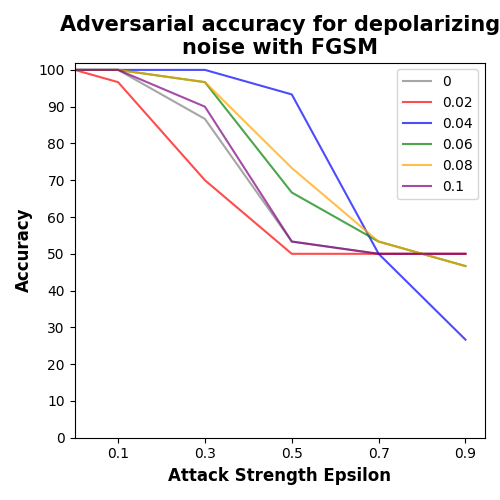
\includegraphics[width=\linewidth]{figures/evaluation_results/iris/pqc/figures/depolarizing-fgsm.png}
      \subcaption{Depolarizing noise model's \ac{fgsm} adversarial accuracy.}
      \label{fig:iris11}
  \end{subfigure} \qquad
  \begin{subfigure}{0.45\textwidth}
      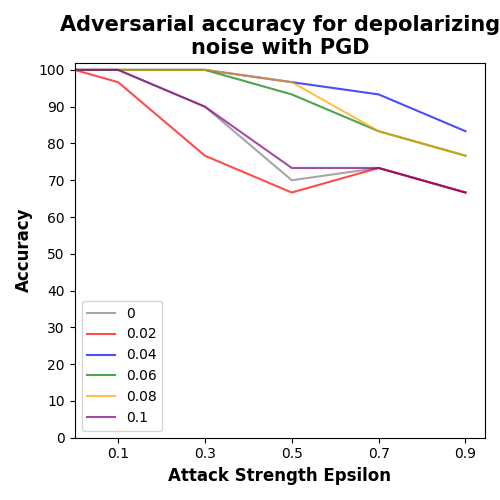
\includegraphics[width=\linewidth]{figures/evaluation_results/iris/pqc/figures/depolarizing-pgd.png}
      \subcaption{Depolarizing noise model's \ac{pgd} adversarial accuracy.}
      \label{fig:iris12}
  \end{subfigure}
  \caption{Depolarizing noise models' accuracy on the adversarial Iris test dataset.}
  \label{fig:iris-1112}
\end{figure} \

In Subfigure~\ref{fig:iris12} we introduce the results from the \ac{pgd}
attack on the depolarizing noisy models. Comparable to the results from
the \ac{fgsm} model evaluation, all models except the one with 2\% noise
probability perform equal or better than the noiseless model throughout
the whole attack strength spectrum. The 4\% noise probability model is
still the best but now doesn't suffer a big drop-off at 0.9 attack strength
like in the \ac{fgsm} outcomes. This model reaches around 83\% adversarial
accuracy with the highest tested attack strength. In this case, although
most of the noisy models have a higher accuracy than the noiseless model,
no correlation can be drawn between model robustness and noise propensity. \

In Figure~\ref{fig:iris-1314} we present the outcomes from the phase damping
noisy models evaluation. For \ac{fgsm} in Subfigure~\ref{fig:iris13}
we note that the models with intermediate noise probabilities (4\% and 6\%)
perform marginally better than the baseline noiseless model up until the
attack strength 0.7. Contrarily, the remaining noise probability models 2\%,
8\% and 10\% obtain a lower adversarial accuracy than the noiseless model.
While some noisy models perform better than the benchmark set by the noiseless
model, no relation between the noise magnitude and the model robustness can
be derived. \

\begin{figure}[!h]
  \centering

  \begin{subfigure}{0.45\textwidth}
      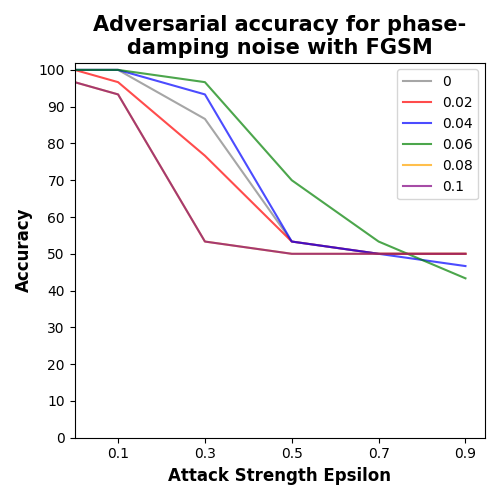
\includegraphics[width=\linewidth]{figures/evaluation_results/iris/pqc/figures/phase-damping-fgsm.png}
      \subcaption{Phase Damping noise model's \ac{fgsm} adversarial accuracy.}
      \label{fig:iris13}
  \end{subfigure} \qquad
  \begin{subfigure}{0.45\textwidth}
      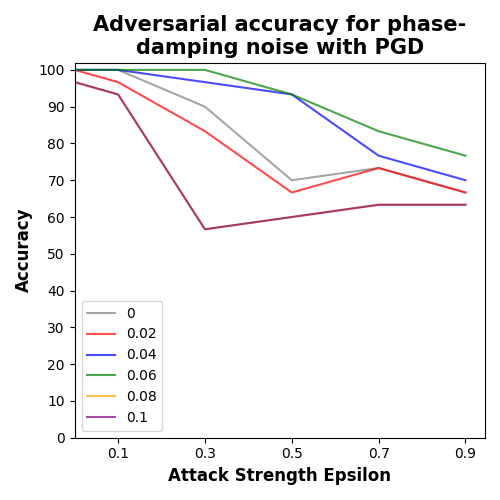
\includegraphics[width=\linewidth]{figures/evaluation_results/iris/pqc/figures/phase-damping-pgd.png}
      \subcaption{Phase Damping noise model's \ac{pgd} adversarial accuracy.}
      \label{fig:iris14}
  \end{subfigure}
  \caption{Phase damping models' accuracy on the adversarial Iris test dataset.}
  \label{fig:iris-1314}
\end{figure} \

In Subfigure~\ref{fig:iris14} we introduce the results from the \ac{pgd}
attack on the phase damping noisy models. The adversarial accuracies
obtained with the \ac{pgd} technique show the same behavior than the
values obtained by the \ac{fgsm} attack. The main difference lies
on the magnitude of the adversarial accuracies, were the results
from the \ac{pgd} tests are slightly higher than for the \ac{fgsm}
experiments. \

In Figure~\ref{fig:iris-1516} we present the outcomes from the phase-flip
noisy models evaluation. For \ac{fgsm} in Subfigure~\ref{fig:iris15}
we note that only the model with the lowest noise probability (2\%)
obtains a higher adversarial accuracy than the baseline noiseless
model. This relationship is maintained up until the 0.7 attack strength,
where the noisy model performance is marginally lower than the noiseless
model. The performance of both types of model, noisy and noiseless,
converges to around 50\% at the highest attack strength. \

\begin{figure}[!h]
  \centering

  \begin{subfigure}{0.45\textwidth}
      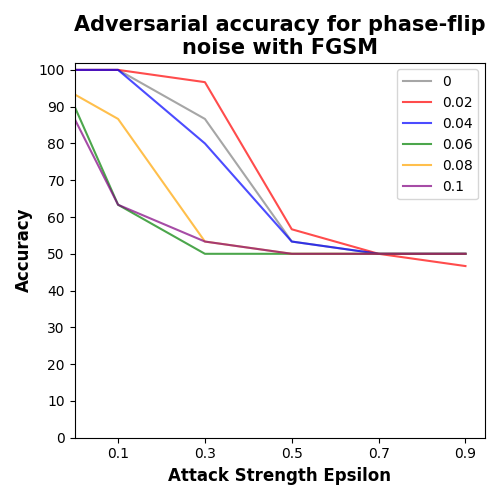
\includegraphics[width=\linewidth]{figures/evaluation_results/iris/pqc/figures/phase-flip-fgsm.png}
      \subcaption{Phase-Flip noise model's \ac{fgsm} adversarial accuracy.}
      \label{fig:iris15}
  \end{subfigure} \qquad
  \begin{subfigure}{0.45\textwidth}
      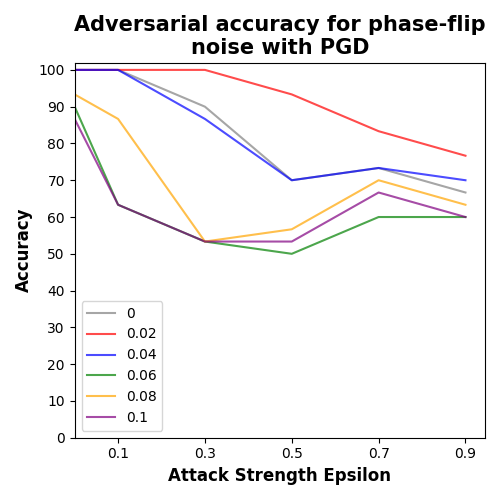
\includegraphics[width=\linewidth]{figures/evaluation_results/iris/pqc/figures/phase-flip-pgd.png}
      \subcaption{Phase-Flip noise model's \ac{pgd} adversarial accuracy.}
      \label{fig:iris16}
  \end{subfigure}

  \caption{Phase-Flip noise models' accuracy on the adversarial Iris test dataset.}
  \label{fig:iris-1516}
\end{figure} \

In Subfigure~\ref{fig:iris16} we introduce the results from the \ac{pgd}
attack on the phase-flip noisy models. Similar to the results from the
\ac{fgsm} attack, only the model with 2\% noise probability performs
better than the noiseless model. Nevertheless, in the case of the \ac{pgd}
adversarial accuracies this behavior is found throughout all the attack
strength range. The performance of the remaining noisy models unexpectedly
either slightly increases or stays the same with increasing attack strength
starting a strength calue of 0.5. For both, the \ac{pgd} and the
\ac{fgsm} attack techniques we can observe a small correlation between the
model robustness, where a higher noise probability equals lesser model
performance. The model with 6\% noise probability is the exception to
this trend because it has the lowest adversarial accuracies throughout
the whole attack strength range. \

\section{\acl{pid} Dataset}\label{section:diabetes-eval} \

The results obtained from training the noisy and noiseless
\ac{qml} models on the \ac{pid} dataset can be found in Subsection
~\ref{subsection:diabetes-noisy-acc}. Moreover, the outcomes
of both adversarial attacks will be presented in Subsection
~\ref{subsection:diabetes-adv-acc}. Finally, the evaluation
of the noisy models against the adversarial attacks can
are presented in Subsection~\ref{subsection:diabetes-noisy-adv-acc}. \

\subsection{Noisy Models Accuracy}\label{subsection:diabetes-noisy-acc} \

In Figure~\ref{fig:diabetes-12} we can observe the results
from the training of noiseless and noisy \ac{qml} models
for the \ac{pid} test dataset. The noiseless baseline model accuracy
can be found on both graphs at the y-intercept, which in
this case is of 67.7\%. We note in Subfigure~\ref{fig:diabetes1}
that for the \ac{pid} dataset the model accuracy slightly decreases
when training with an increasing coherent noise effect. The model
performance is slowly reduced until it reaches 49\% accuracy. \

For incoherent noise models in Subfigure~\ref{fig:diabetes2}
we can observe a decrease in model accuracy for all the noise
models. In this case, phase damping noise performs the best
of any noise models, followed then by models with amplitude
damping noise. They each have an accuracy of 59\% and 49\% on the clean
test dataset respectively, which represents a lower performance
than the noiseless model's accuracy. \

Regarding the bit-flip, depolarizing, and phase-flip noise, the model
performance significantly decreases its accuracy to 44\% starting at
4\% noise probability and remains at that same value for all
higher noise probabilities. Interestingly enough, there seems
to not be any relation between which type of incoherent noise
is used and the performance of the model. While in the Iris
dataset (Subfig.~\ref{fig:iris2}) the best performing models
were the ones using bit-flip and depolarizing noise, in the
\ac{pid} dataset phase and amplitude damping noise have the
highest accuracy. \

\begin{figure}[!h]
  \centering

  \begin{subfigure}{0.45\textwidth}
      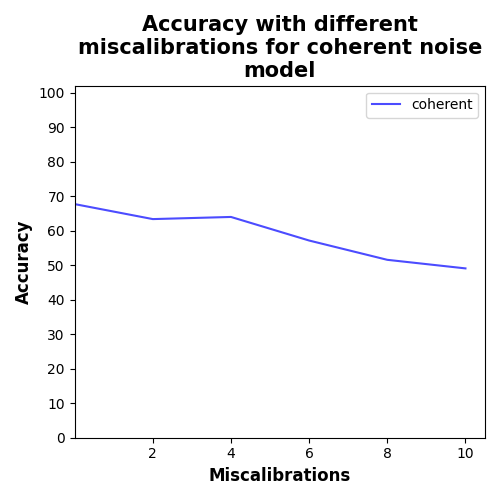
\includegraphics[width=\linewidth]{figures/evaluation_results/diabetes/pqc/figures/accuracy-coherent.png}
      \subcaption{Coherent noise model's accuracy.}
      \label{fig:diabetes1}
  \end{subfigure} \qquad
  \begin{subfigure}{0.45\textwidth}
      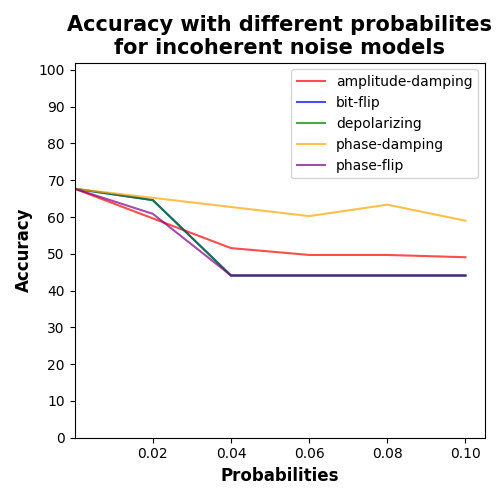
\includegraphics[width=\linewidth]{figures/evaluation_results/diabetes/pqc/figures/accuracy-incoherent.png}
      \subcaption{Incoherent noise models' accuracy.}
      \label{fig:diabetes2}
  \end{subfigure}

  \caption{\ac{vqa}'s accuracy on the \ac{pid} clean test dataset.}
  \label{fig:diabetes-12}
\end{figure} \

\subsection{Adversarial Accuracy}\label{subsection:diabetes-adv-acc} \

In Figure~\ref{fig:diabetes-34} we introduce the effects of the
adversarial attacks on the accuracy of the noiseless \ac{qml}
model. As expected, we can observe that for both adversarial
techniques the performance of the model decreases with increasing
attack strength. For both of the adversarial techniques
we notice a stark accuracy decrease until it stabilizes to around
\(33\%\) after \(0.3\) attack strength. That \ac{fgsm} (Subfig.
~\ref{fig:diabetes3}) has the same performance impact as \ac{pgd}
(Subfigure~\ref{fig:diabetes4}) is not expected, as \ac{fgsm}'s
perturbations tend to be bigger in magnitude and more disruptive
to the input. \

\begin{figure}[!h]
  \centering

  \begin{subfigure}{0.45\textwidth}
      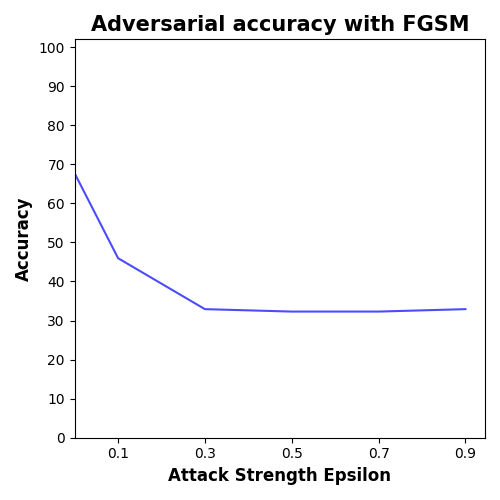
\includegraphics[width=\linewidth]{figures/evaluation_results/diabetes/pqc/figures/none-fgsm.png}
      \subcaption{Noiseless model's \ac{fgsm} adversarial accuracy.}
      \label{fig:diabetes3}
  \end{subfigure} \qquad
  \begin{subfigure}{0.45\textwidth}
      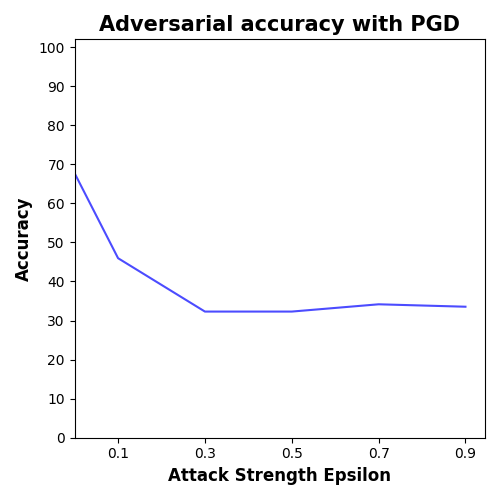
\includegraphics[width=\linewidth]{figures/evaluation_results/diabetes/pqc/figures/none-pgd.png}
      \subcaption{Noiseless model's \ac{pgd} adversarial accuracy.}
      \label{fig:diabetes4}
  \end{subfigure}

  \caption{\ac{vqa}'s accuracy on the adversarial \ac{pid} test dataset.}
  \label{fig:diabetes-34}
\end{figure} \

\subsection{Noisy Models Adversarial Accuracy}\label{subsection:diabetes-noisy-adv-acc} \

In this subsection we introduce the results from performing
the adversarial attacks on the noisy models with different noise
magnitudes for the \ac{pid} dataset. In each graph the color gray
represents the baseline adversarial accuracy obtained by the
noiseless model. \

In Figure~\ref{fig:diabetes-56} we present the outcomes from the amplitude
damping noisy models evaluation. For \ac{fgsm} in Subfigure~\ref{fig:diabetes5}
we note that \

\begin{figure}[!h]
  \centering

  \begin{subfigure}{0.45\textwidth}
      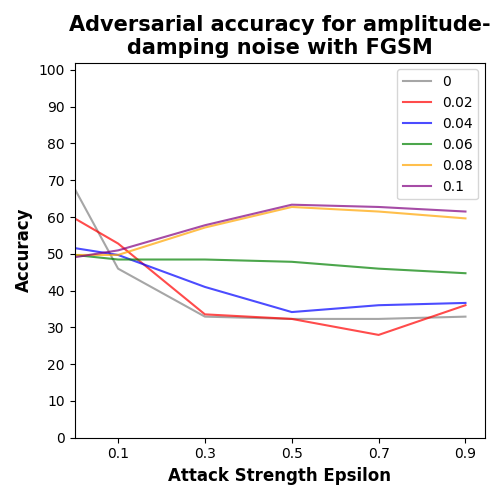
\includegraphics[width=\linewidth]{figures/evaluation_results/diabetes/pqc/figures/amplitude-damping-fgsm.png}
      \subcaption{Amplitude damping noise model's \ac{fgsm} adversarial accuracy.}
      \label{fig:diabetes5}
  \end{subfigure} \qquad
  \begin{subfigure}{0.45\textwidth}
      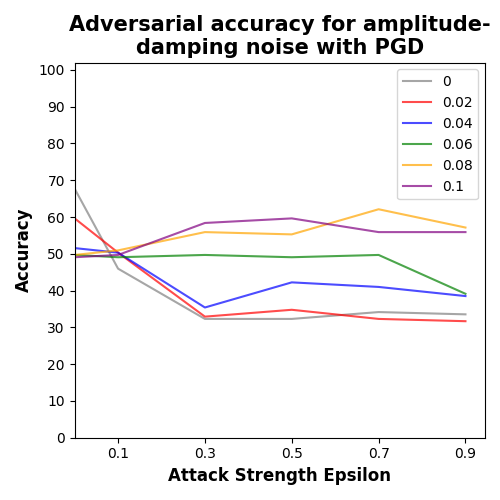
\includegraphics[width=\linewidth]{figures/evaluation_results/diabetes/pqc/figures/amplitude-damping-pgd.png}
      \subcaption{Amplitude damping noise model's \ac{pgd} adversarial accuracy.}
      \label{fig:diabetes6}
  \end{subfigure}
  \caption{Amplitude damping noise models' accuracy on the adversarial \ac{pid} test dataset.}
  \label{fig:diabetes-56}
\end{figure} \

In Subfigure~\ref{fig:diabetes6} we introduce the results from the \ac{pgd}
attack on the amplitude damping noisy models. \

In Figure~\ref{fig:diabetes-78} we present the outcomes from the bit-flip
noisy models evaluation. For \ac{fgsm} in Subfigure~\ref{fig:diabetes7}
we note that \

\begin{figure}[!h]
  \centering

  \begin{subfigure}{0.45\textwidth}
      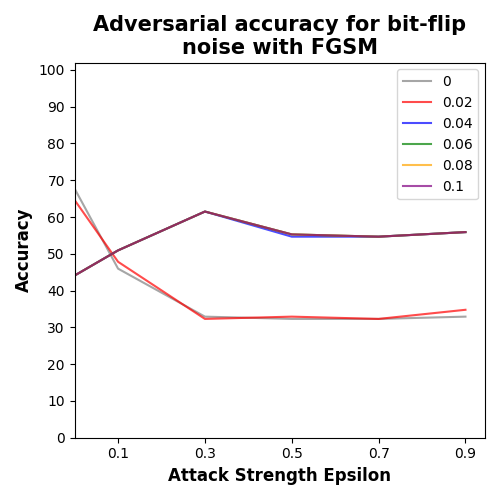
\includegraphics[width=\linewidth]{figures/evaluation_results/diabetes/pqc/figures/bit-flip-fgsm.png}
      \subcaption{Bit-Flip noise model's \ac{fgsm} adversarial accuracy.}
      \label{fig:diabetes7}
  \end{subfigure} \qquad
  \begin{subfigure}{0.45\textwidth}
      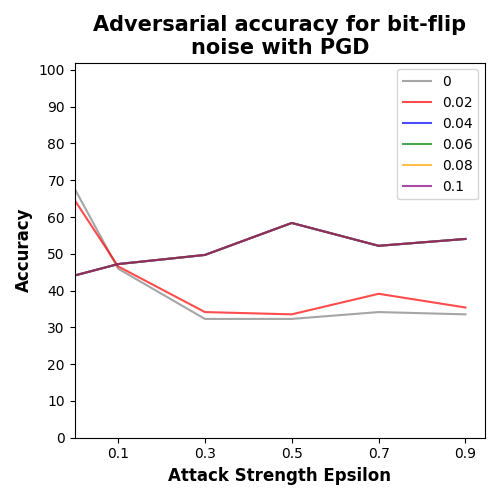
\includegraphics[width=\linewidth]{figures/evaluation_results/diabetes/pqc/figures/bit-flip-pgd.png}
      \subcaption{Bit-Flip noise model's \ac{pgd} adversarial accuracy.}
      \label{fig:diabetes8}
  \end{subfigure}
  \caption{Bit-Flip noise models' accuracy on the adversarial \ac{pid} test dataset.}
  \label{fig:diabetes-78}
\end{figure} \

In Subfigure~\ref{fig:diabetes8} we introduce the results from the \ac{pgd}
attack on the bit-flip noisy models. \

In Figure~\ref{fig:diabetes-910} we present the outcomes from the coherent
noisy models evaluation. For \ac{fgsm} in Subfigure~\ref{fig:diabetes9}
we note that \

\begin{figure}[!h]
  \centering

  \begin{subfigure}{0.45\textwidth}
      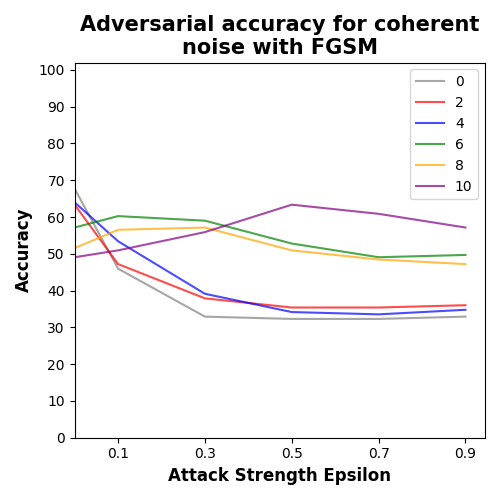
\includegraphics[width=\linewidth]{figures/evaluation_results/diabetes/pqc/figures/coherent-fgsm.png}
      \subcaption{Coherent noise model's \ac{fgsm} adversarial accuracy.}
      \label{fig:diabetes9}
  \end{subfigure} \qquad
  \begin{subfigure}{0.45\textwidth}
      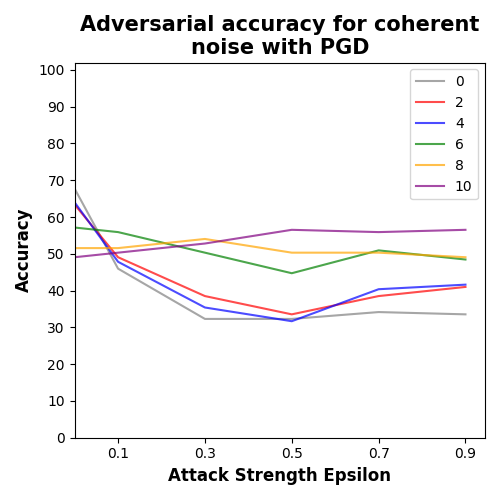
\includegraphics[width=\linewidth]{figures/evaluation_results/diabetes/pqc/figures/coherent-pgd.png}
      \subcaption{Coherent noise model's \ac{pgd} adversarial accuracy.}
      \label{fig:diabetes10}
  \end{subfigure}
  \caption{Coherent noise models' accuracy on the adversarial \ac{pid} test dataset.}
  \label{fig:diabetes-910}
\end{figure} \

In Subfigure~\ref{fig:diabetes10} we introduce the results from the \ac{pgd}
attack on the coherent noisy models. \

In Figure~\ref{fig:diabetes-1112} we present the outcomes from the depolarizing
noisy models evaluation. For \ac{fgsm} in Subfigure~\ref{fig:diabetes11}
we note that \

\begin{figure}[!h]
  \centering

  \begin{subfigure}{0.45\textwidth}
      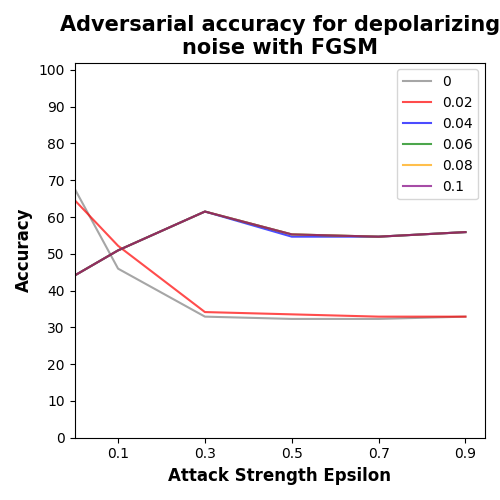
\includegraphics[width=\linewidth]{figures/evaluation_results/diabetes/pqc/figures/depolarizing-fgsm.png}
      \subcaption{Depolarizing noise model's \ac{fgsm} adversarial accuracy.}
      \label{fig:diabetes11}
  \end{subfigure} \qquad
  \begin{subfigure}{0.45\textwidth}
      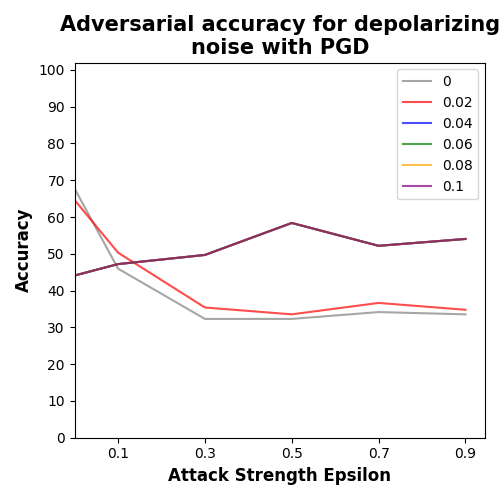
\includegraphics[width=\linewidth]{figures/evaluation_results/diabetes/pqc/figures/depolarizing-pgd.png}
      \subcaption{Depolarizing noise model's \ac{pgd} adversarial accuracy.}
      \label{fig:diabetes12}
  \end{subfigure}
  \caption{Depolarizing noise models' accuracy on the adversarial \ac{pid} test dataset.}
  \label{fig:diabetes-1112}
\end{figure} \

In Subfigure~\ref{fig:diabetes12} we introduce the results from the \ac{pgd}
attack on the depolarizing noisy models. \

In Figure~\ref{fig:diabetes-1314} we present the outcomes from the phase damping
noisy models evaluation. For \ac{fgsm} in Subfigure~\ref{fig:diabetes13}
we note that \

\begin{figure}[!h]
  \centering

  \begin{subfigure}{0.45\textwidth}
      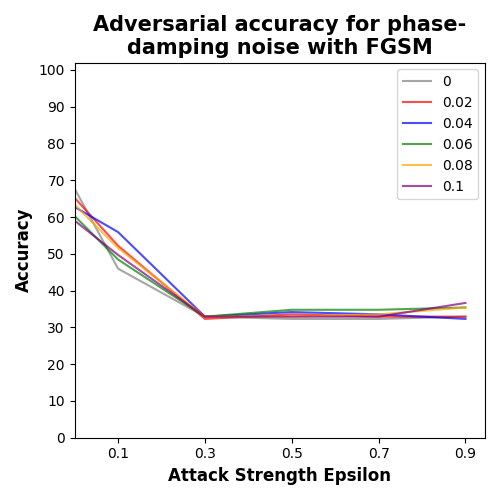
\includegraphics[width=\linewidth]{figures/evaluation_results/diabetes/pqc/figures/phase-damping-fgsm.png}
      \subcaption{Phase Damping noise model's \ac{fgsm} adversarial accuracy.}
      \label{fig:diabetes13}
  \end{subfigure} \qquad
  \begin{subfigure}{0.45\textwidth}
      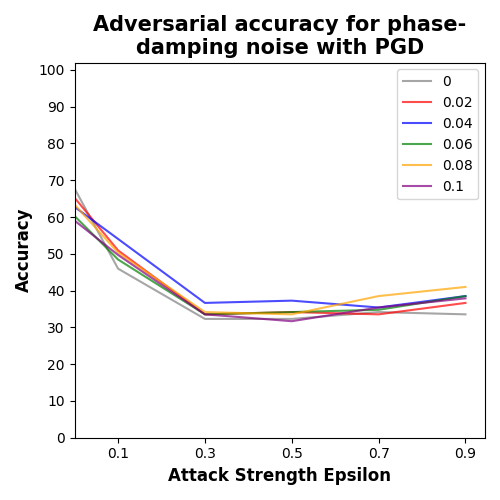
\includegraphics[width=\linewidth]{figures/evaluation_results/diabetes/pqc/figures/phase-damping-pgd.png}
      \subcaption{Phase Damping noise model's \ac{pgd} adversarial accuracy.}
      \label{fig:diabetes14}
  \end{subfigure}
  \caption{Phase damping models' accuracy on the adversarial \ac{pid} test dataset.}
  \label{fig:diabetes-1314}
\end{figure} \

In Subfigure~\ref{fig:diabetes14} we introduce the results from the \ac{pgd}
attack on the phase damping noisy models. \

In Figure~\ref{fig:diabetes-1516} we present the outcomes from the phase-flip
noisy models evaluation. For \ac{fgsm} in Subfigure~\ref{fig:diabetes15}
we note that \

\begin{figure}[!h]
  \centering

  \begin{subfigure}{0.45\textwidth}
      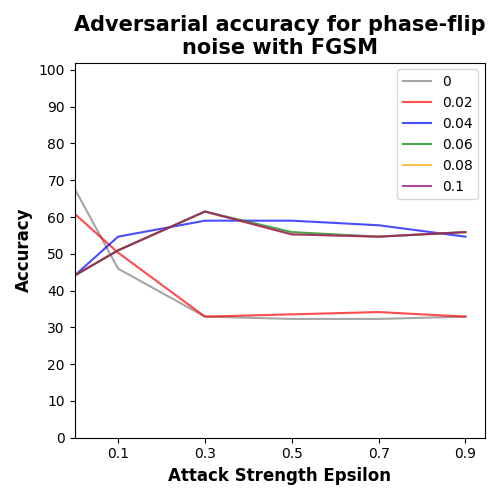
\includegraphics[width=\linewidth]{figures/evaluation_results/diabetes/pqc/figures/phase-flip-fgsm.png}
      \subcaption{Phase-Flip noise model's \ac{fgsm} adversarial accuracy.}
      \label{fig:diabetes15}
  \end{subfigure} \qquad
  \begin{subfigure}{0.45\textwidth}
      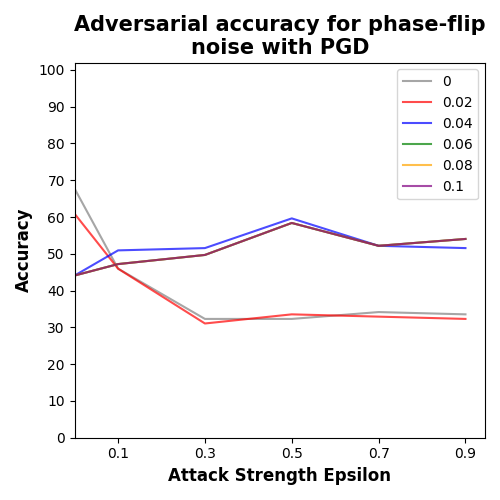
\includegraphics[width=\linewidth]{figures/evaluation_results/diabetes/pqc/figures/phase-flip-pgd.png}
      \subcaption{Phase-Flip noise model's \ac{pgd} adversarial accuracy.}
      \label{fig:diabetes16}
  \end{subfigure}

  \caption{Phase-Flip noise models' accuracy on the adversarial \ac{pid} test dataset.}
  \label{fig:diabetes-1516}
\end{figure} \

In Subfigure~\ref{fig:diabetes16} we introduce the results from the \ac{pgd}
attack on the phase-flip noisy models. \

\section{Breast Cancer Dataset}\label{section:breast-cancer-eval} \

\subsection{Noisy Models Accuracy}\label{subsection:breast-cancer-noisy-acc} \

\subsection{Adversarial Accuracy}\label{subsection:breast-cancer-adv-acc} \

\subsection{Noisy Models Adversarial Accuracy}\label{subsection:breast-cancer-noisy-adv-acc} \

In this subsection we introduce the results from performing
the adversarial attacks on the noisy models with different noise
magnitudes for the Wisconsin Breast Cancer dataset. In each graph
the color gray represents the baseline adversarial accuracy obtained
by the noiseless model. \

In Figure~\ref{fig:bc-56} we present the outcomes from the amplitude
damping noisy models evaluation. For \ac{fgsm} in Subfigure~\ref{fig:bc5}
we note that \

\begin{figure}[!h]
  \centering

  \begin{subfigure}{0.45\textwidth}
      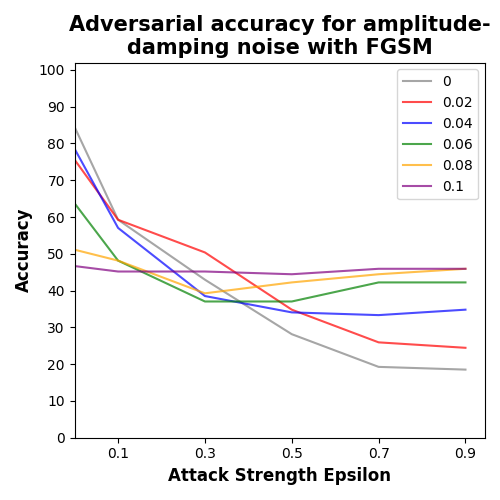
\includegraphics[width=\linewidth]{figures/evaluation_results/breast-cancer/pqc/figures/amplitude-damping-fgsm.png}
      \subcaption{Amplitude damping noise model's \ac{fgsm} adversarial accuracy.}
      \label{fig:bc5}
  \end{subfigure} \qquad
  \begin{subfigure}{0.45\textwidth}
      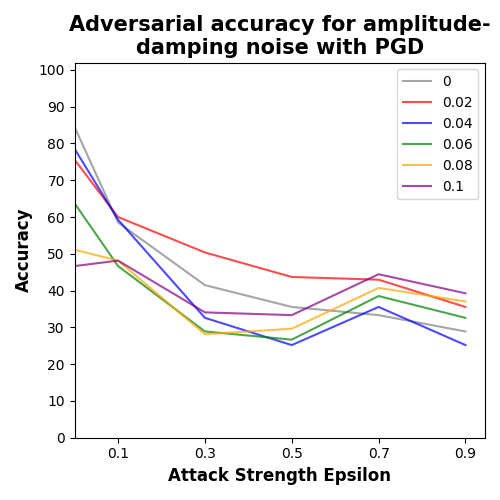
\includegraphics[width=\linewidth]{figures/evaluation_results/breast-cancer/pqc/figures/amplitude-damping-pgd.png}
      \subcaption{Amplitude damping noise model's \ac{pgd} adversarial accuracy.}
      \label{fig:bc6}
  \end{subfigure}
  \caption{Amplitude damping noise models' accuracy on the adversarial Wisconsin Breast Cancer test dataset.}
  \label{fig:bc-56}
\end{figure} \

In Subfigure~\ref{fig:bc6} we introduce the results from the \ac{pgd}
attack on the amplitude damping noisy models. \

In Figure~\ref{fig:bc-78} we present the outcomes from the bit-flip
noisy models evaluation. For \ac{fgsm} in Subfigure~\ref{fig:bc7}
we note that \

\begin{figure}[!h]
  \centering

  \begin{subfigure}{0.45\textwidth}
      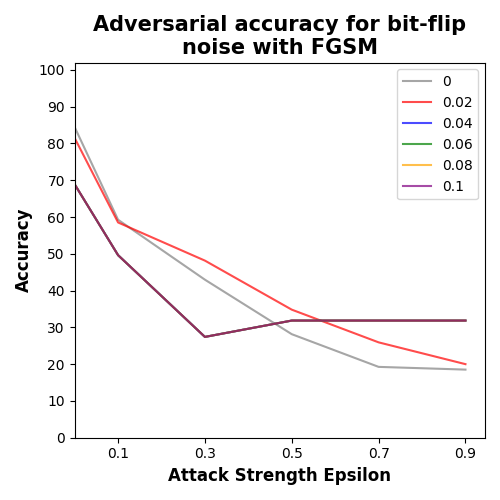
\includegraphics[width=\linewidth]{figures/evaluation_results/breast-cancer/pqc/figures/bit-flip-fgsm.png}
      \subcaption{Bit-Flip noise model's \ac{fgsm} adversarial accuracy.}
      \label{fig:bc7}
  \end{subfigure} \qquad
  \begin{subfigure}{0.45\textwidth}
      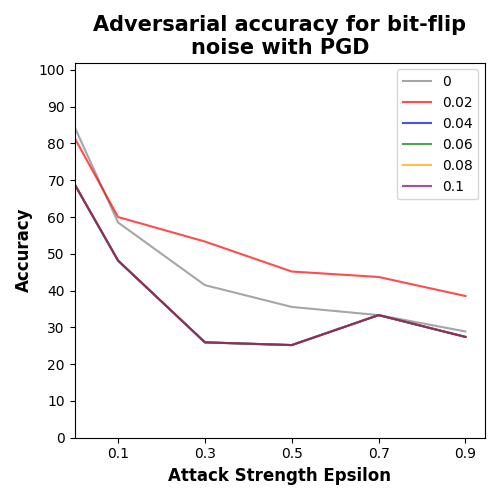
\includegraphics[width=\linewidth]{figures/evaluation_results/breast-cancer/pqc/figures/bit-flip-pgd.png}
      \subcaption{Bit-Flip noise model's \ac{pgd} adversarial accuracy.}
      \label{fig:bc8}
  \end{subfigure}
  \caption{Bit-Flip noise models' accuracy on the adversarial Wisconsin Breast Cancer test dataset.}
  \label{fig:bc-78}
\end{figure} \

In Subfigure~\ref{fig:bc8} we introduce the results from the \ac{pgd}
attack on the bit-flip noisy models. \

In Figure~\ref{fig:bc-910} we present the outcomes from the coherent
noisy models evaluation. For \ac{fgsm} in Subfigure~\ref{fig:bc9}
we note that \

\begin{figure}[!h]
  \centering

  \begin{subfigure}{0.45\textwidth}
      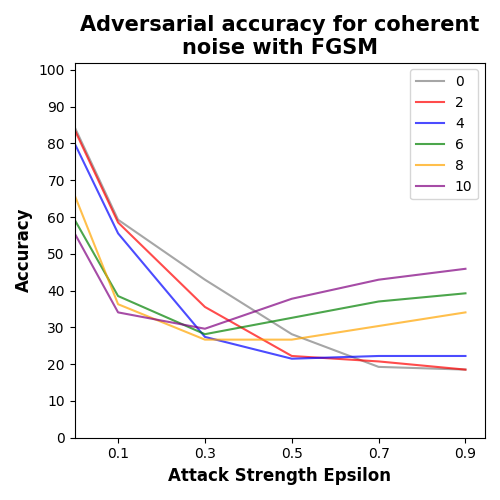
\includegraphics[width=\linewidth]{figures/evaluation_results/breast-cancer/pqc/figures/coherent-fgsm.png}
      \subcaption{Coherent noise model's \ac{fgsm} adversarial accuracy.}
      \label{fig:bc9}
  \end{subfigure} \qquad
  \begin{subfigure}{0.45\textwidth}
      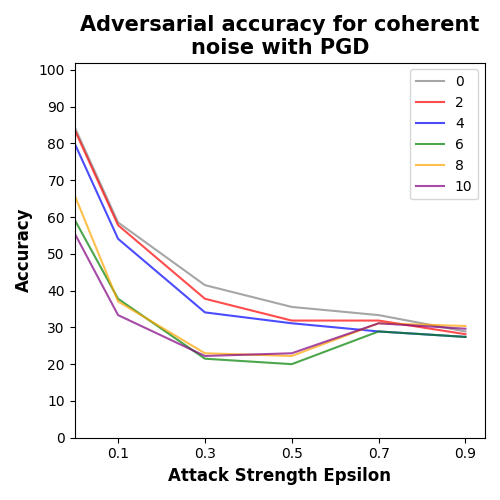
\includegraphics[width=\linewidth]{figures/evaluation_results/breast-cancer/pqc/figures/coherent-pgd.png}
      \subcaption{Coherent noise model's \ac{pgd} adversarial accuracy.}
      \label{fig:bc10}
  \end{subfigure}
  \caption{Coherent noise models' accuracy on the adversarial Wisconsin Breast Cancer test dataset.}
  \label{fig:bc-910}
\end{figure} \

In Subfigure~\ref{fig:bc10} we introduce the results from the \ac{pgd}
attack on the coherent noisy models. \

In Figure~\ref{fig:bc-1112} we present the outcomes from the depolarizing
noisy models evaluation. For \ac{fgsm} in Subfigure~\ref{fig:bc11}
we note that \

\begin{figure}[!h]
  \centering

  \begin{subfigure}{0.45\textwidth}
      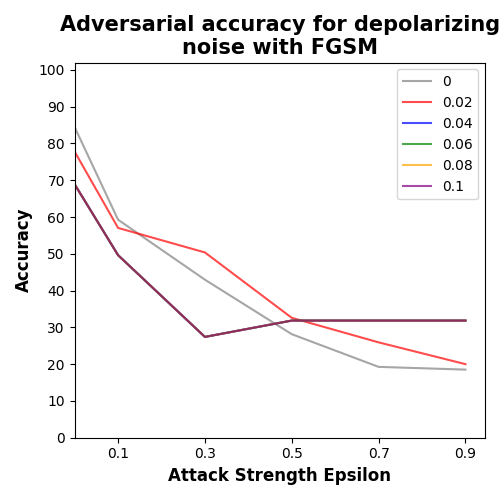
\includegraphics[width=\linewidth]{figures/evaluation_results/breast-cancer/pqc/figures/depolarizing-fgsm.png}
      \subcaption{Depolarizing noise model's \ac{fgsm} adversarial accuracy.}
      \label{fig:bc11}
  \end{subfigure} \qquad
  \begin{subfigure}{0.45\textwidth}
      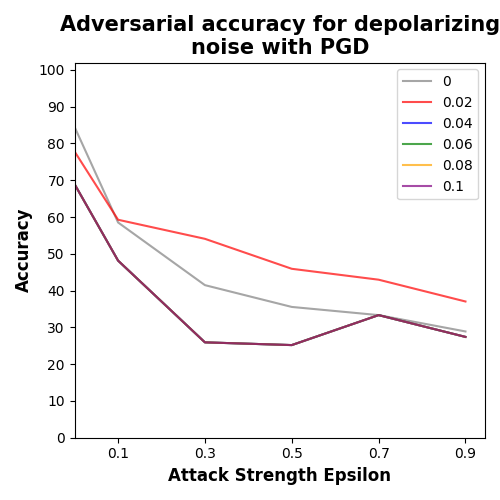
\includegraphics[width=\linewidth]{figures/evaluation_results/breast-cancer/pqc/figures/depolarizing-pgd.png}
      \subcaption{Depolarizing noise model's \ac{pgd} adversarial accuracy.}
      \label{fig:bc12}
  \end{subfigure}
  \caption{Depolarizing noise models' accuracy on the adversarial Wisconsin Breast Cancer test dataset.}
  \label{fig:bc-1112}
\end{figure} \

In Subfigure~\ref{fig:bc12} we introduce the results from the \ac{pgd}
attack on the depolarizing noisy models. \

In Figure~\ref{fig:bc-1314} we present the outcomes from the phase damping
noisy models evaluation. For \ac{fgsm} in Subfigure~\ref{fig:bc13}
we note that \

\begin{figure}[!h]
  \centering

  \begin{subfigure}{0.45\textwidth}
      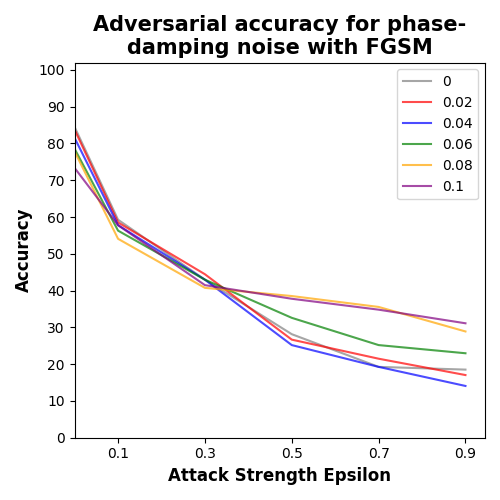
\includegraphics[width=\linewidth]{figures/evaluation_results/breast-cancer/pqc/figures/phase-damping-fgsm.png}
      \subcaption{Phase Damping noise model's \ac{fgsm} adversarial accuracy.}
      \label{fig:bc13}
  \end{subfigure} \qquad
  \begin{subfigure}{0.45\textwidth}
      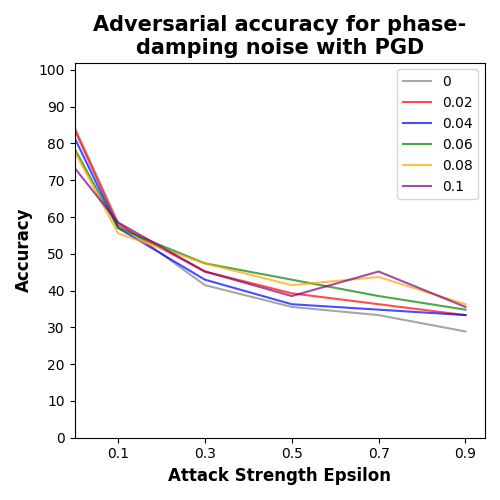
\includegraphics[width=\linewidth]{figures/evaluation_results/breast-cancer/pqc/figures/phase-damping-pgd.png}
      \subcaption{Phase Damping noise model's \ac{pgd} adversarial accuracy.}
      \label{fig:bc14}
  \end{subfigure}
  \caption{Phase damping models' accuracy on the adversarial Wisconsin Breast Cancer test dataset.}
  \label{fig:bc-1314}
\end{figure} \

In Subfigure~\ref{fig:bc14} we introduce the results from the \ac{pgd}
attack on the phase damping noisy models. \

In Figure~\ref{fig:bc-1516} we present the outcomes from the phase-flip
noisy models evaluation. For \ac{fgsm} in Subfigure~\ref{fig:bc15}
we note that \

\begin{figure}[!h]
  \centering

  \begin{subfigure}{0.45\textwidth}
      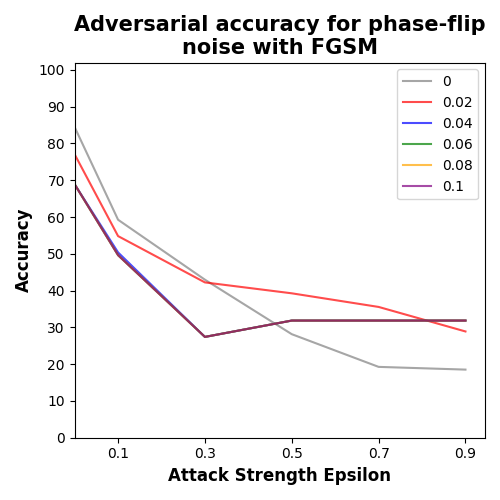
\includegraphics[width=\linewidth]{figures/evaluation_results/breast-cancer/pqc/figures/phase-flip-fgsm.png}
      \subcaption{Phase-Flip noise model's \ac{fgsm} adversarial accuracy.}
      \label{fig:bc15}
  \end{subfigure} \qquad
  \begin{subfigure}{0.45\textwidth}
      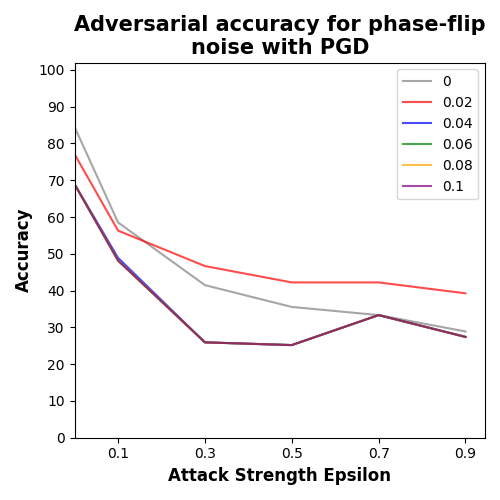
\includegraphics[width=\linewidth]{figures/evaluation_results/breast-cancer/pqc/figures/phase-flip-pgd.png}
      \subcaption{Phase-Flip noise model's \ac{pgd} adversarial accuracy.}
      \label{fig:bc16}
  \end{subfigure}

  \caption{Phase-Flip noise models' accuracy on the adversarial Wisconsin Breast Cancer test dataset.}
  \label{fig:bc-1516}
\end{figure} \

In Subfigure~\ref{fig:bc16} we introduce the results from the \ac{pgd}
attack on the phase-flip noisy models. \

\section{Plus-Minus Dataset}\label{section:plus-minus-eval} \

\subsection{Noisy Models Accuracy}\label{subsection:plus-minus-noisy-acc} \

\subsection{Adversarial Accuracy}\label{subsection:plus-minus-adv-acc} \

\subsection{Noisy Models Adversarial Accuracy}\label{subsection:plus-minus-noisy-adv-acc} \

\subsection{Discussion}\label{subsection:discussion} \

PGD results might vary as the iterative process will result in different
values every time. \

Iris dataset might be too simple on clean dataset. (probs not if it is being affected by the adversarial attacks)

Coherent noise might just work as a bias term on the clean dataset? \

Iris dataset notes: \

Amplitude damping works worse than baseline, no relation between noise
probability and adv accuracy. \

bit-flip, some models perform better than baseline but no relationship
between noise probability and adv accuracy can be found. \

for pgd with bit-flip and amplitude damping the performance gets better
for some models with increased attack strength. \

coherent noise seems to increase model robustness, specially at higher noise
probabilities, maybe works as a bias term that better enables the model
to adjust the classification threshold. \

depolarizing noise is in general better in both attacks than the baseline
model but no conclusions can be drawns. \

phase-damping: main diff between pgd and fgsm is the accuracy levels,
were fgsm affects reduces more the accuracy than pgd. this applies to
all noisy models, so there isn't a different noisy model behavior
depending on the adv attack, just a change in the adv acc values. \

phase-flip: slight correlation found between noise probs and robustness,
it is an inverse relationship, meaning that the higher the noise the worse
the performance.


1.	Explain why decoherent noise is used and not coherent. \

  a. Coherent noise will probably just shift the bias. \

  b. Coherent noise might add too much noise (quadratic growth). \

  c. True random noise is required to improve generalization. \

% TODO: Do an experiment implementing coherent noise to prove this claim.
% Use https://pennylane.ai/qml/demos/tutorial_variational_classifier/ - circuit-centric quantum classifier ansatz

\section{Variational Quantum Algorithm Model Accuracy}\label{section:vqa_accuracy} \

% TODO: State the result of training QVC with regards to the chosen datasets.
% TODO: Compare to paper and state why they might be valid results.

\section{Variational Quantum Algorithm Model Adversarial Accuracy}\label{section:vqa_adversarial_accuracy} \

% TODO: Present results per dataset of the different attacks and attack strengths